\subsection{Introduction}
%\addcontentsline{toc}{subsection}{Introduction}
The study investigates the relative strengths of various Lewis acids and bases by calculating the binding energies of their adducts and analyzing key factors influencing these interactions. Specifically, adducts formed between boron and aluminum based hydrides and halides as Lewis acids, nitrogen and phosphorus containing bases were examined using \textit{ab-initio} quantum mechanical methods. The same methodology and calculations from project 1 were performed with a different basis set Hartree-Fock HF 3-21G in Gaussian 16, with visualization in GaussView 6.

The relative acid and base strengths were evaluated through chemical hardness, determined from HOMO and LUMO energies. Additional parameters analyzed include vertical electron attachment energy, reorganization energy, proton affinity, and partial atomic charges on donor and acceptor atoms. Steric and electronic interactions were further explored by visualizing HOMO-LUMO orbital overlaps.

%Theory
\subsection{Theory}
%\addcontentsline{toc}{subsection}{Theory}
\subsubsection{Lewis acid and base}
\begin{itemize}
    \item \textbf{Lewis acid} is an electron pair acceptor. It possesses an empty orbital, often resulting from an electron-deficient central atom or a positive charge, which enables it to accept a pair of electrons from another species. This makes Lewis acids Electrophilic in nature, and they commonly have incomplete octets as in 13th Boron and Aluminum complexes. They have low energy LUMO orbital to accept electrons from HOMO of base.
    \item \textbf{Lewis base} is an electron pair donor. It has at least one lone pair of electrons available for donation, enabling it to form a coordinate covalent bond with a Lewis acid. Lewis bases are thus Nucleophilic, and typically feature atoms such as nitrogen, oxygen, or phosphorus with non-bonding electron pairs. They have high energy HOMO to donate electron to acids.
    \item \textbf{Acid–Base adduct} is a chemical compound formed when a Lewis base donates a lone pair of electrons to a Lewis acid, resulting in a coordinate covalent bond.
\end{itemize}

\subsubsection{Binding Energy}
Binding Energy ($\Delta E_{bind}$) is the energy difference between the adduct and the sum of the energies of the separate acid and base. For a gas-phase reaction between a Lewis acid and a
Lewis base, The binding energy is given by:

\[
\mathrm{A(g)} + \mathrm{:B(g)} \rightarrow \mathrm{A{:}B(g)}
\]
\[
\Delta E_{bind} = E_{A:B} - (E_{A} \;+ \; E_{B})
\]
\[
If \; \Delta E_{bind} < 0 	\Rightarrow Exothermic \;  and \;  Thermodynamically \; favourable
\]
\[
If \; \Delta E_{bind} > 0 	\Rightarrow Endothermic \;  and \;  Thermodynamically \; unfavourable
\]


\subsubsection{Factors Affecting Binding Energy}
A negative binding energy doesn't guarantee Lewis acid–base adduct formation, as factors like kinetics, sterics, and acid–base compatibility (e.g., hard–hard interactions) also influence binding. Here, we explore the key factors affecting adduct stability and binding energy.

\paragraph{i). Energies of HOMO and LUMO}~
\begin{itemize}
    \item A higher energy Highest Occupied Molecular Orbital(HOMO), closer to 0 eV or less negative means more willing to donate electrons. Therefore, a base with a high HOMO is considered a stronger Lewis base.
    \item A lower energy Lowest unoccupied Molecular Orbital (LUMO), more negative means more favorable to accept electrons. Therefore, an acid with a low LUMO is considered a stronger Lewis acid.
\end{itemize}
\paragraph{ii). Hardness of acid and base}
The Hardness is the concept which measures the strength of lewis acid and base and classify them as hard and soft. The hardness $(\eta)$ scale used here is Parr–Pearson Hardness (or Density Functional Theory-DFT Global Hardness) can be formulated as:
\[
\eta = \frac{E_{\text{LUMO}} - E_{\text{HOMO}}}2
\]
$Large \; \eta \Rightarrow $  Soft acid and base $\Rightarrow$ Species which resist change in electron density and less reactive. 

$Small \; \eta \Rightarrow $  Hard acid and base $\Rightarrow$ Species which more polarisable and more reactive.

\paragraph{iii). Reorganizational Energy of idealised acid: }
It is the energy required to change the geometry of the acid from trigonal planar to the idealized pyramidal structure. The geometry change happens when an acid interact with base during the formation of adduct.
\[
E_{reorg} = E_{planar} - E_{idealised \; pyramidal}
\]


\paragraph{iv). Reorganizational Energy of acid and base in adduct}
The base is removed from the adduct, and the energy of the acid in the geometry it adopts within the adduct, \( E_{AB}^{A} \), is calculated. The \textbf{reorganizational energy of the acid} is then given by \(  E_{AB}^{A} - E_0^A \), where \( E_0^A \) is the energy of the free acid at its own optimized geometry.

Similarly, the acid is removed from the adduct, and the energy of the base in the geometry it adopts within the adduct, \( E_{AB}^{B} \), is calculated. The \textbf{reorganizational energy of the base} is given by \( E_{AB}^{B} - E_0^B \), where \( E_0^B \) is the energy of the free base at its optimized geometry.

\paragraph{v). Vertical Electron Attachment Energy (VEAE) of acid}~
It is the energy change when an electron is added to a molecule without allowing the molecule to change its geometry. The geometry of acid remains same for both the structures, either planar or idealized pyramidal.
\[
E_{VEAE} = E_{pyamidal \; MX_3 } - E_{pyamidal \; MX_3^- } 
\]

\paragraph{vi). Proton affinity of base}~
It is a measure of the tendency of a base to accept a proton $(H^+)$ in the gas phase. It is proportional with the basicity of a molecule.

\[
\text{B (g)} + \text{H}^+ \rightarrow \text{BH}^+ \text{ (g)} \qquad \text{PA} = -\Delta H
\]
\[
\Delta H_{PA} = (\Delta H_{Base} +  \Delta H_{H^{+}}) -  \Delta H_{(Base-H)^{+}} 	\simeq \Delta H_{Base} -  \Delta H_{(Base-H)^{+}}
\]

\paragraph{vii). Charge transfer on adduct formation}~
It is the extent of net Mulliken charge transfer from base to acid in an adduct. It is the charge difference on the donor atom in its isolated state and in adduct. It can be formulated as:
\[
\Delta Q_{BA} = q_{isolated} \;-\; q_{adduct}
\]


\paragraph{viii). Change in the M–X bond distance in the acid}
\[
\Delta r_{MX} = \text{M-X bond length  of acid in adduct} - \text{M-X bond length  of free acid}
\]

\paragraph{ix). X–M–X bond angle in the acid of the adduct}
The \( \angle XMX\)  is the angle between the central and the substituent atoms. In a free acid with idealized pyramidal geometry, the angle is \( 109^\circ 50^{\prime\prime}\). But due to adduct formation, the \( \angle XMX\) changes and it can be observed in \cref{adduct_table}.


\paragraph{x). Electrostatic and steric interactions}~
Steric and electronic interactions refer to the repulsion caused by bulky groups surrounding the acceptor and donor centers of a Lewis acid or base. These interactions can hinder the close approach required for effective orbital overlap and reduce or prevent adduct formation. Even when the electronic properties like hardness, HOMO $\&$ LUMO energy levels favor adduct formation, steric hindrance can distort geometry and lower the stability or block the interaction entirely. This can be observed for 2,6-dimethylpyridine–\ce{BCl_3} adduct in \cref{adduct_table}, which despite involving one of the strongest Lewis acid-base pairs, exhibits lower binding energy compared to complexes such as \ce{NH_3}-\ce{AlCl_3} and 3,5-dimethylpyridine–\ce{BCl_3}. The reduced stability is attributed to steric hindrance from the methyl groups at the 2' and 6' positions of the pyridine ring, which prevents effective interaction with the Lewis acid.
\vspace{1em}

\textbf{Unit Conversion:}
\[
1 \;Hatree = 1 \;a.u.= 27.2114 \;eV= 627.509 \;kcal/mol = 2625.50\;kJ/mol
\]


\newpage
%Observation and Results
%\addcontentsline{toc}{subsection}{Observation and Results}
\subsection{Observation}
\label{project2}

\renewcommand{\arraystretch}{2}
\begin{table}[H]
\centering
\begin{tabular}{|>{\centering\arraybackslash}m{2cm}
                |>{\centering\arraybackslash}m{1.5cm}
                |>{\centering\arraybackslash}m{1.5cm}
                |>{\centering\arraybackslash}m{2cm}
                |>{\centering\arraybackslash}m{2cm}
                |>{\centering\arraybackslash}m{2cm}
                |>{\centering\arraybackslash}m{1.5cm}|}
\hline
\textbf{Molecule} & \textbf{$E_{HOMO}$ (eV)} & \textbf{$E_{LUMO}$ (eV)} & \textbf{Hardness (eV)} & \textbf{$\Delta E_{\mathrm{EA}^{a}}$ (kcal/mol)} & \textbf{$\Delta E_{\mathrm{reorg}}^{b}$ (kcal/mol)} & $Q_{AA}^{c}$ (statC) \\
\hline
\textbf{BH$_3$ }  & -12.87 & 1.15  & 7.01 & 8.29   & 24.37 & 0.03 \\
\hline
\textbf{BF$_3$  } & -16.96 & 0.47  & 8.72 & -5.65  & 46.18 & 1.19 \\
\hline
\textbf{BCl$_3$}  & -12.85 & -1.39 & 5.73 & -63.76 & 40.66 & 0.31 \\
\hline
\textbf{AlH$_3$ } & -11.28 & -0.02 & 5.63 & -13.91 & 20.69 & 0.76 \\
\hline
\textbf{AlCl$_3$} & -12.79 & -2.29 & 5.25 & -68.45 & 21.12 & 1.39 \\
\hline
\end{tabular}
\caption{Calculated Properties of the Idealized Pyramidal Boron and Aluminum
Hydrides and Halides using \textit{HF 3-21G basis set}}
\label{acid_table}
\end{table}

\renewcommand{\arraystretch}{1.5}
\begin{table}[H]
\centering
\begin{tabular}{|>{\centering\arraybackslash}m{4cm}
                |>{\centering\arraybackslash}m{1.5cm}
                |>{\centering\arraybackslash}m{1.5cm}
                |>{\centering\arraybackslash}m{2cm}
                |>{\centering\arraybackslash}m{2cm}
                |>{\centering\arraybackslash}m{1.5cm}|}
\hline
\textbf{Lewis base }& \textbf{$E_{\mathrm{HOMO}}$ (eV)} & \textbf{$E_{\mathrm{LUMO}}$ (eV)} &\textbf{ Hardness (eV)} &\textbf{ Proton Affinity (PA) (kcal/mol)} & $Q_{DA}^{d}$ (statC) \\
\hline
\textbf{NF$_3$ }& -15.01 & 6.02 & 10.52 & 126.24 & 0.65 \\
\hline
\textbf{PH$_3$ }& -10.36 & 4.93 & 7.64 & 184.27 & 0.09 \\
\hline
\textbf{NH$_3$ }& -10.59 & 7.49 & 9.04 & 226.94 & -0.88 \\
\hline
\textbf{Pyridine} & -9.69 & 3.54 & 6.61 & 241.22 & -0.67 \\
\hline
\textbf{3,5-Dimethylpyridine} & -9.13 & 3.56 & 6.34 & 246.06 & -0.68 \\
\hline
\textbf{N(CH$_3$)$_3$} & -9.08 & 6.92 & 8.00 & 248.03 & -0.68 \\
\hline
\textbf{2,6-Dimethylpyridine} & -9.08 & 3.62 & 6.35 & 250.04 & -0.75 \\
\hline
\end{tabular}
\caption{ Calculated Properties of the Lewis Bases using \textit{HF 3-21G basis set}}
\label{base_table}
\end{table}


$^{\mathrm{a}}$ Vertical electron attachment energy that occurs when an electron is added to the neutral \chemfig{MX_3} molecule at the idealized pyramidal geometry.\\
$^{\mathrm{b}}$ The re-organizational energy necessary to change the geometry of the
acid from trigonal planar to the idealized pyramidal structure.\\
$^{\mathrm{c}}$ The partial charge on the acceptor atom.\\
$^{\mathrm{d}}$ Partial charge on the donor atom \\

\newpage
\renewcommand{\arraystretch}{2}
\begin{table}[!htp]
\centering
\begin{tabular}{|>{\centering\arraybackslash}m{2.5cm}
                |>{\centering\arraybackslash}m{1.2cm}
                |>{\centering\arraybackslash}m{1cm}
                |>{\centering\arraybackslash}m{1cm}
                |>{\centering\arraybackslash}m{1.5cm}
                |>{\centering\arraybackslash}m{1.4cm}
                |>{\centering\arraybackslash}m{1.4cm}
                |>{\centering\arraybackslash}m{1cm}
                |>{\centering\arraybackslash}m{1cm}
                |>{\centering\arraybackslash}m{1cm}|}
\hline
\textbf{Adduct} & $\Delta BE^{a}$ (kcal mol$^{-1}$) & $r_{MN}^{b}$ (\AA) & $r_{MX}^{c}$ (\AA) & $\angle XMX^{d}$ ($^\circ$) & $E_\text{reorg acid}^{e}$ (kcal mol$^{-1}$) & $E_\text{reorg base}^{f}$ (kcal mol$^{-1}$) & $\Delta Q_{BA}^{g}$ & $\Delta Q_{DA}^{h}$ & $Q_{AA}^{i}$ \\
\hline
H$_3$N:AlCl$_3$ & -66.98 & 1.98 & 0.04 & 116.50 & 6.61 & 0.54 & 0.25 & -1.01 & 1.40 \\
\hline
H$_3$N:BCl$_3$ & -49.14 & 1.63 & 0.10 & 113.50 & 24.98 & 0.40 & 0.36 & -0.90 & 0.27 \\
\hline
H$_3$N:AlH$_3$ & -42.88 & 2.05 & 0.02 & 116.86 & 5.42 & 0.33 & 0.19 & -0.96 & 0.74 \\
\hline
H$_3$N:BF$_3$ & -42.09 & 1.69 & 0.05 & 114.13 & 24.11 & 0.20 & 0.20 & -0.98 & 1.19 \\
\hline
H$_3$N:BH$_3$ & -35.65 & 1.71 & 0.02 & 113.95 & 13.59 & 0.22 & 0.26 & -0.86 & 0.00 \\
\hline
H$_3$P:AlCl$_3$ & -27.27 & 2.54 & 0.04 & 116.74 & 6.11 & 2.56 & 0.14 & -0.04 & 1.43 \\
\hline
H$_3$P:AlH$_3$ & -12.69 & 2.72 & 0.01 & 118.67 & 2.23 & 0.85 & 0.05 & 0.00 & 0.80 \\
\hline
H$_3$P:BH$_3$ & -8.39 & 2.21 & 0.01 & 116.80 & 6.96 & 1.07 & 0.27 & 0.24 & -0.18 \\
\hline
H$_3$P:BCl$_3$ & -7.73 & 2.06 & 0.10 & 113.85 & 23.76 & 4.33 & 0.66 & 0.49 & -0.16 \\
\hline
H$_3$P:BF$_3$ & -5.70 & 3.03 & 0.00 & 119.74 & 0.90 & 0.17 & 0.01 & 0.02 & 1.20 \\
\hline
3,5-Dimethyl-pyridine:BCl$_3$ & -47.92 & 1.61 & 0.12 & 111.07 & 33.72 & 0.65 & 0.36 & -0.96 & 0.35 \\
\hline
pyridine:BCl$_3$ & -46.68 & 1.61 & 0.12 & 111.24 & 33.01 & 0.69 & 0.35 & -0.94 & 0.35 \\
\hline
2,6-Dimethyl-pyridine:BCl$_3$ & -28.66 & 1.62 & 0.13 & 111.49 & 42.20 & 10.83 & -0.36 & -1.00 & 0.35 \\
\hline
\end{tabular}
\caption{Calculated properties of Ammonia and Phosphine adducts of Lewis acid using \textit{HF 3-21G basis set.}}
\label{adduct_table}
\end{table}


$^{\mathrm{a}}$ Binding energy. \\
$^{\mathrm{b}}$ Donor atom-acceptor atom bond distance in the adduct.\\
$^{\mathrm{c}}$ Change in the M-X bond distance in the acid of the adduct.\\
$^{\mathrm{d}}$ Value of the X-M-X bond angle in the acid of the adduct.\\
$^{\mathrm{e}}$ Re-organizational energy of the acid upon adduct formation as a result of a change in the structure.\\
$^{\mathrm{f}}$ Re-organizational energy of the acid upon adduct formation as a result of a change in the structure.\\
$^{\mathrm{g}}$ Net Mulliken Charge transfer from the base to the acid upon adduct formation.\\
$^{\mathrm{h}}$ Charge on the donor atom of the base in the adduct.\\
$^{\mathrm{i}}$ Charge on the acceptor atom of the acid in the adduct.\\


%Figures

%\newpage
% For Printout
% \begin{figure}[htp]
%     \centering
%     \fbox{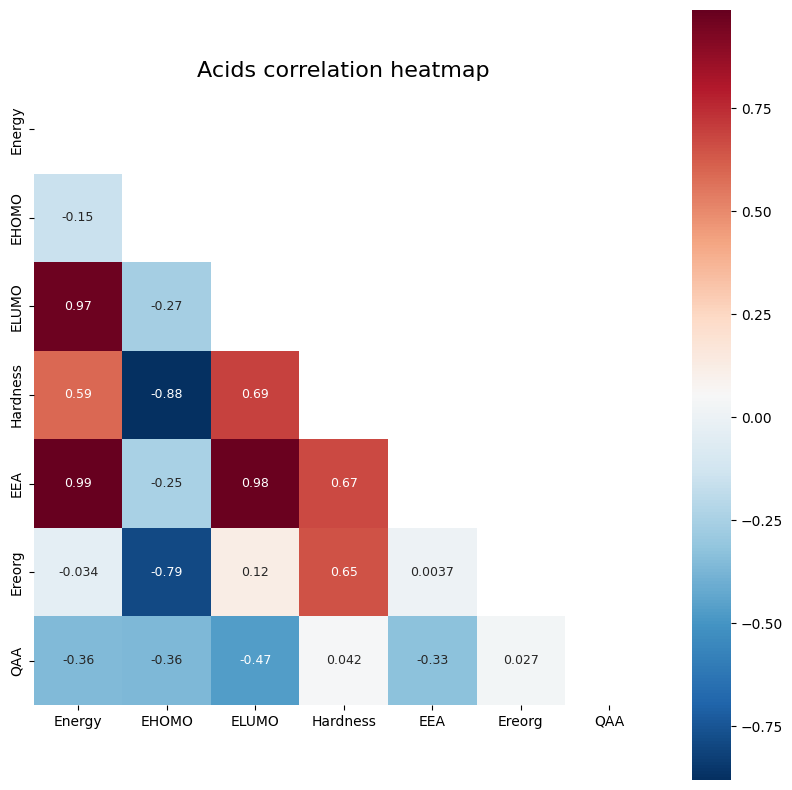
\includegraphics[width=16cm, height=7.5cm]{Acid_Base/images/acid_heatmap.png}}
%     \caption{Heatmap with corelation coefficient showing relation between different quantitative variables of Acids}
%     \label{fig:Acid_heatmap}
% \end{figure}
% \begin{figure}[htp]
%     \centering
%     \fbox{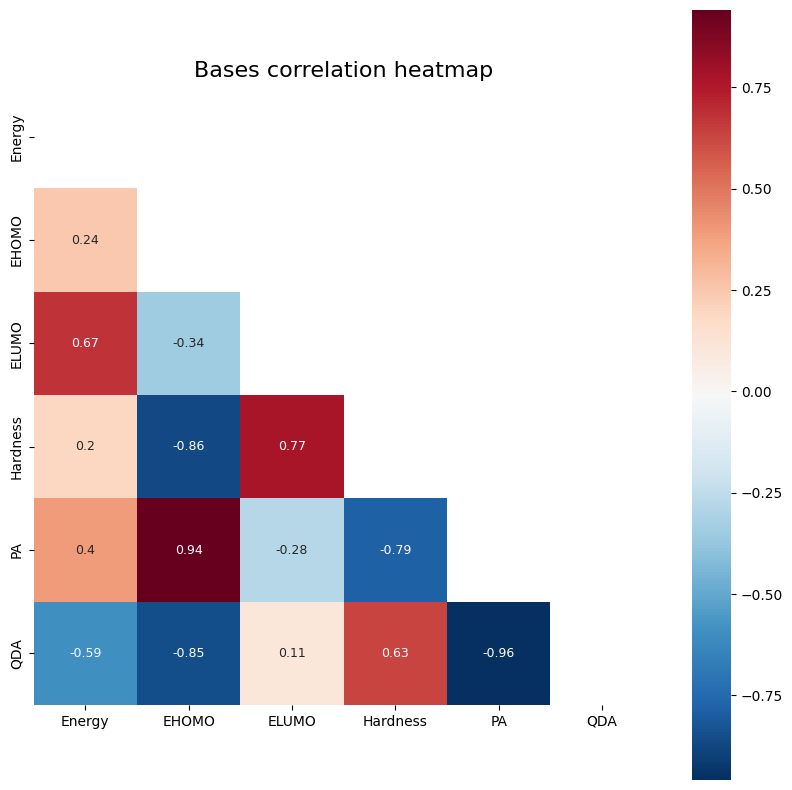
\includegraphics[width=16cm, height=7.5cm]{Acid_Base/images/base_heatmap.png}}
%     \caption{Heatmap with corelation coefficient showing relation between different quantitative variables of Bases}
%     \label{fig:Base_heatmap}
% \end{figure}

% For online PDF
\newpage
\begin{figure}[H]
    \centering
    \fbox{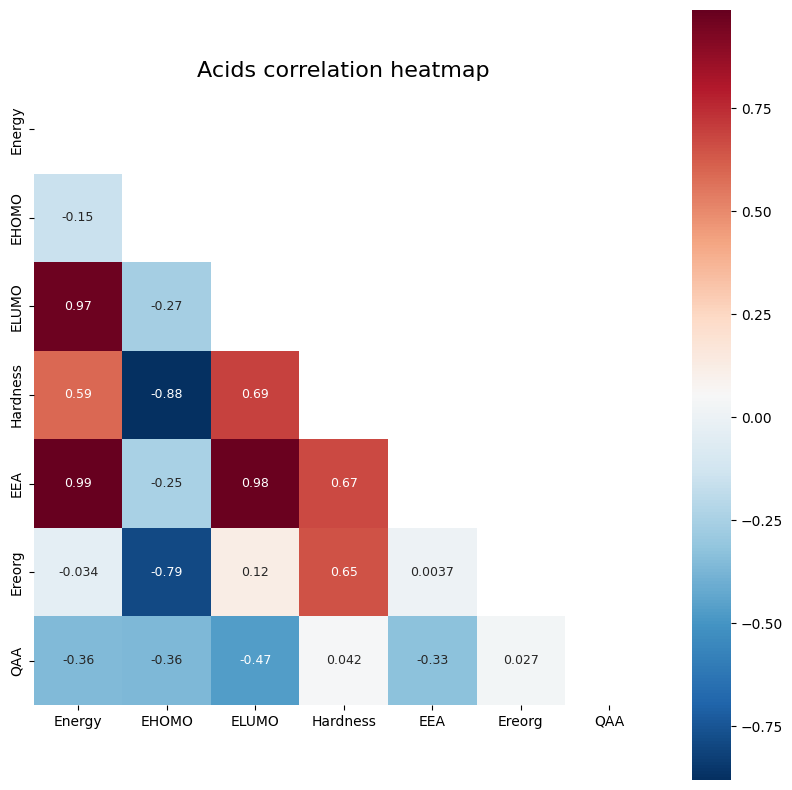
\includegraphics[width=\textwidth]{Acid_Base/images/acid_heatmap.png}}
    \caption{Heatmap with corelation coefficient showing relation between different quantitative variables of Acids}
    \label{fig:Acid_heatmap}
\end{figure}

\newpage
\begin{figure}[H]
    \centering
    \fbox{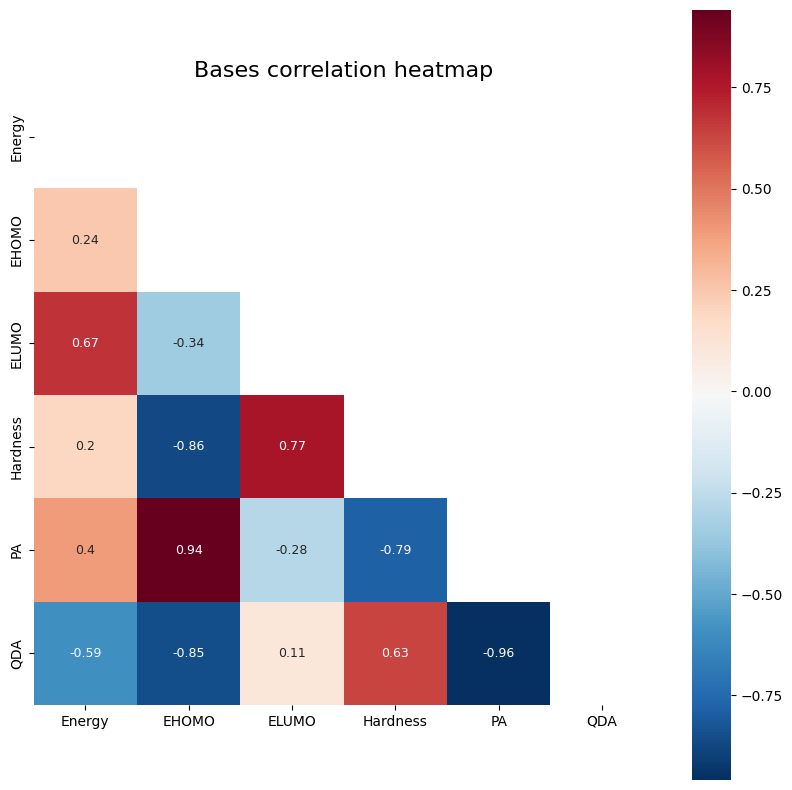
\includegraphics[width=\textwidth]{Acid_Base/images/base_heatmap.png}}
    \caption{Heatmap with corelation coefficient showing relation between different quantitative variables of Bases}
    \label{fig:Base_heatmap}
\end{figure}

\begin{figure}[H]
    \centering
    % First image
    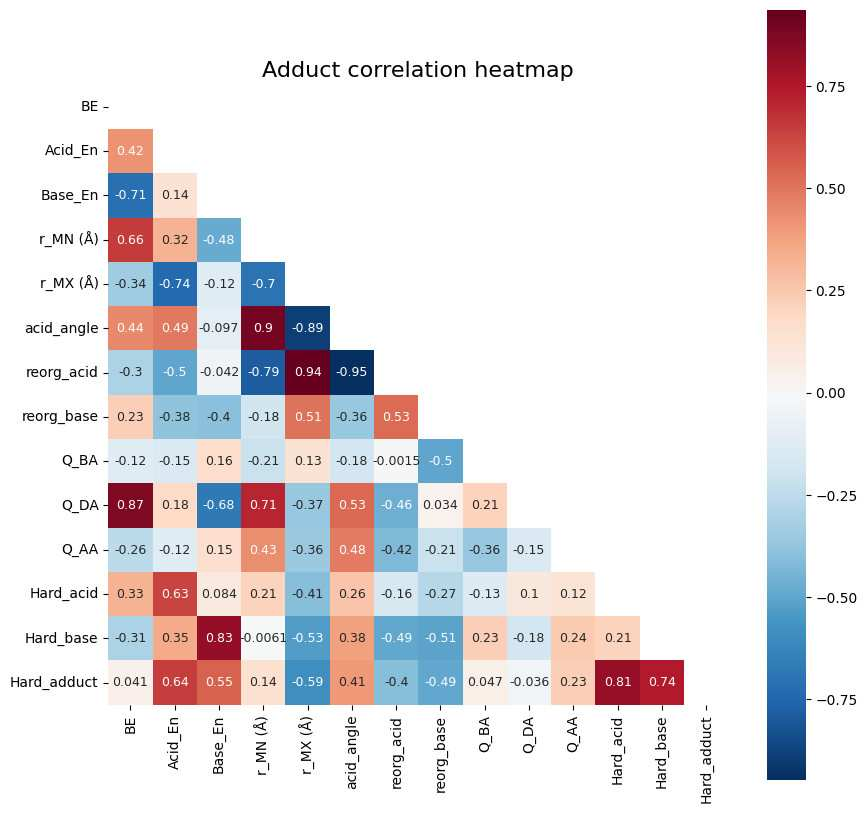
\includegraphics[width=0.9\linewidth]{Acid_Base/images/adduct_heatmap.jpeg}
    \caption{Heatmap with corelation coefficient showing relation between different quantitative variables of Acid-Base adducts}
    \label{fig:adduct-heatmap}

    \vspace{1em} % Vertical space between images

    % Side-by-side images
    \begin{minipage}[b]{0.48\linewidth}
        \centering
        \fbox{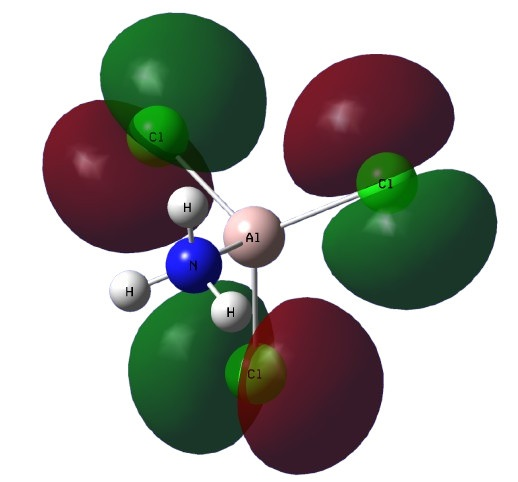
\includegraphics[width=\linewidth]{Acid_Base/images/NH3_AlCl3_homo.jpeg}
        \caption*{(a) $NH_3-AlCl_3$ adduct HOMO}}
    \end{minipage}
    \hfill
    \begin{minipage}[b]{0.48\linewidth}
        \centering
        \fbox{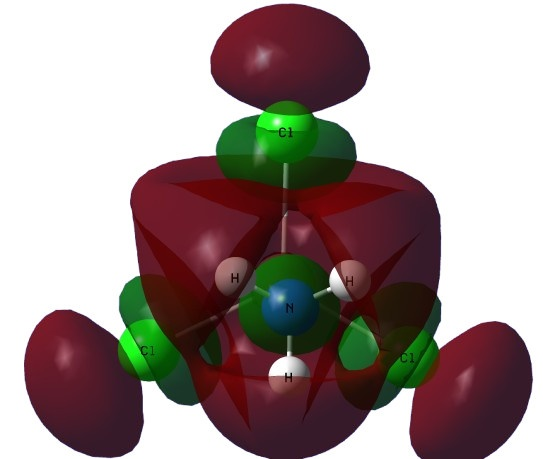
\includegraphics[width=\linewidth]{Acid_Base/images/NH3_AlCl3_lumo.jpeg}
        \caption*{(b) $NH_3-AlCl_3$ adduct LUMO}}
    \end{minipage}
    %\caption{Side-by-side comparison of two figures.}
    %\label{fig:side-by-side}
\end{figure}

\newpage
%Discussion
\subsection{Results}
%\addcontentsline{toc}{subsection}{Discussion}
\subsubsection{Strength of acid, base and adducts}
From the observation of hardness value of acids from \cref{acid_table}, the descending order of the strength of acid can be given as:
\[AlCl{_3} > AlH_3 > BCl_3 > BH_3 > BF_3 \]
From the observation of hardness value of acids from \cref{base_table}, the descending order of the strength of base can be given as:
\[ 3,5-dimethylpyridine \simeq 2,6-dimethylpyridine > pyridine > PH_3 > N(CH_3)_3 > NH_3 > NF_3 \]
From observation of the binding energy value of the Lewis acid ammonia and phosphorus adducts of \cref{adduct_table}, the descending order of the strength of the adducts can be given as:
\begin{align*}
& NH_3\text{–}AlCl_3 > NH_3\text{–}BCl_3 > 3,5\text{-dimethylpyridine–}BCl_3 > \text{pyridine–}BCl_3 > \\
& NH_3\text{–}AlH_3 > NH_3\text{–}BF_3 > NH_3\text{–}BH_3 > PH_3\text{–}AlCl_3 > \\
& 2,6\text{-dimethylpyridine–}BCl_3 > PH_3\text{–}AlH_3 > PH_3\text{–}BH_3 > PH_3\text{–}BCl_3 > PH_3\text{–}BF_3
\end{align*}

\subsubsection{Correlation Heatmap}
A correlation heatmap is a data visualization technique that uses color to represent Pearson's correlation coefficient (r) in a 2D matrix. The value of the correlation coefficient ranges from 1 to -1.
\begin{align*}
r &= +1 \Rightarrow \text{Perfect positive linear correlation (all points lie exactly on a line with positive slope)} \\
r &\in (0, 1) \Rightarrow \text{Weak to strong positive linear correlation with deviations from straight line} \\
r &= 0 \Rightarrow \text{No linear or non-linear correlation} \\
r &\in (-1, 0) \Rightarrow \text{Weak to strong negative linear correlation with deviations from straight line} \\
r &= -1 \Rightarrow \text{Perfect negative linear correlation (all points lie exactly on a line with negative slope)}
\end{align*}


From the acid correlation heat map shown in \cref{fig:Acid_heatmap}, we can visualize the relationship between different factors affecting the hardness of acid. We can write the following conclusion from it.
\[
Strength \propto \frac{1}{Hardness} \propto \frac{1}{E_{LUMO}} \propto E_{HOMO}  \propto \frac{1}{E_{EA}} \propto \frac{1}{E_{reorg}} \propto \frac{1}{Energy}
\]

From the base correlation heat map shown in \cref{fig:Base_heatmap}, we can visualize the relationship between different factors affecting the hardness of base. We can write the following conclusion from it.
\[
Strength \propto \frac{1}{Hardness} \propto \frac{1}{E_{LUMO}} \propto E_{HOMO} \propto \Delta E_{PA}  \propto \frac{1}{Q_{DA}}
\]

\newpage
From the adduct correlation heat map shown in \cref{fig:adduct-heatmap}, we can visualize the relationship between different factors that affect the hardness of the Ammonia and Phosphine adducts of Lewis acid. From this we can draw the following conclusion.
\[
\Delta E_{bind} \propto \frac{1}{E_{base}} \propto Q_{DA} \propto r_{MN} \propto \angle XMX \propto E_{acid}
\]
\[
r_{MX} \propto \Delta E_{reorg \; acid} \propto \frac{1}{\angle XMX}
\]
\[
r_{MN} \propto \angle XMX \propto Q_{DA} \propto \frac{1}{\Delta E_{reorg \; base}} \propto \frac{1}{r_{MX}}
\]


%Conclusion
\subsection{Discussion and Conclusion}
%\addcontentsline{toc}{subsection}{Conclusion}
This study demonstrated that \textit{ab-initio single point Hatree Fock HF/3-21G} calculations effectively capture trends in Lewis acid-base adducts binding energies and related electronic properties. The Key parameters such as $E_{LUMO}, E_{HOMO} ,$ hardness, and proton affinity were consistent with higher-level data from literature (Anderson, 2000), confirming the method’s reliability for qualitative analysis.

Overall, this work provides a foundation for future studies involving more complex systems or higher levels of theory. The ability to predict and interpret acid-base behavior computationally is a powerful tool for guiding experimental design and advancing theoretical understanding in coordination chemistry, catalysis, and materials science.\\


\noindent\dotfill

\newpage
